\chapter{Présentation des API}

\section{Facebook}
\subsection{Aperçu général du réseau social Facebook}

Facebook est un réseau social en ligne qui permet l'échange à plusieurs niveaux entre ses utilisateurs. Mise à part le fait qu'il soit le deuxième site wen le plus visité au monde, il est aussi le réseau social qui compte le plus d'utilisateurs. En effet, Facebook a 968 millions d'utilisateurs actifs au quotidiens sur un total de 1,46 milliard d'utilisateurs actifs mensuels.
Facebook est né en 2004 à Harvard. Reservé au début aux étudiants de l'université Harvard et ensuite ouvert à d'autres universités américaines, il devient accesible à tous en 2006. Le nom du site provient du mot trombinoscope communément appelé facebook en anglais. 
Initiallement, Facebook a été crée pour permettre la mise en relation entre ses utilisateurs.Cet aspect demeure le noyau du réseau social mais néaumoins pas le seul. En effet, au fil des années, de nouvelles et multiples fonctionnalités se sont rajoutées. Parmi ces dernières, les plus importantes à citer sont : 
\begin{itemize}
\item $follow$ : suivre une personne ou une page et consulter ses publications publiques.
\item $like$ : aimer des publications (photo, vidéo, évenement, article et autre).
\item $share$ : partager les diverses types de publications possibles.
\item $post$ : toute personne inscrite à Facebook, peut poster des publications. Ces dernières peuvent être soit des photos, vidéos, événements, article, des URL et autres.
\end{itemize}
On accède au site web de Facebook en tapant : \url{www.facebook.com}. Il faut évidement s'inscrire pour accéder à l'ensemble des optionalités qu'offre Facebook.\\
Outre ce qui est mentionné ci-dessus, Facebook offre une platforme. Elle permet aux développeurs de logger leurs utilisateurs via leurs compte Facebook. Ce système requiert l'API de Facebook et une application crée par le développeur. Le système Graph, détaillé ultérieurement et qui permet de récupérer les informations relatives à l'utilisateur Facebook, peut être utilisé. Cette platforme est accesible via : \url{https://developers.facebook.com}.

\subsection{Open Graph API}


Facebook fournit une API qui est l'Open Graph API. Cette API permet l'accès à des objets et des connexions ) du graphe social de Facebook communément appelé $Social$ $Graph$.\\
Dans le $Social$ $Graph$ de Facebook, chaque $Object$ représente un noeud. Un objet peut présenter une personne, un article, une page Facebook, des articles de presse ou encore des morceaux de musiques, un groupe Facebook voire même une application. Les objets sont liés entre eux par des actions.
Aisi, le $Social$ $Graph$ est un protocole qui permet à des sites tiers d'interagir avec les informations d'un profil Facebook et avec les relations de ce dernier. Ces informations sont appelées objets, puisque sur Facebook, les utilisateurs sont connectés à leurs relations sociales, mais également à des objets.\\
L'Open Graph n'est autre que la traduction de la politique de Facebook de vouloir mettre autant d'informations à disposition des développeurs afin de leur permettre la création d'application ainsi qu'offrir une palette d'opportunités aux sites tiers pour faire du Facebook Connect un identifiant web unique.\\
Un profil Facebook n'est pas une simple carte d'identité, c'est un profil social intégrant la totalité des informations et celles des relations d'un profil donné. L'Open Graph est donc un ensemble de métadonnées, qui grandissent au fil de son intégration sur des sites tiers. N'importe quel éditeur pourra alors les exploiter dès que l'internaute se connecte sur son site avec le Facebook Connect.\\
l'Open Graph rassemble toutes les informations concernant l'activité d'une personne dès que celle-ci est connectée à un site via le Facebook Connect. En plus de savoir ce que une personne fait lorsqu'elle est connectée, il permet à l'utilisateur de savoir ce que ses amis font, aiment, lisent, partagent etc.

\begin{figure}[!h]
\begin{center}
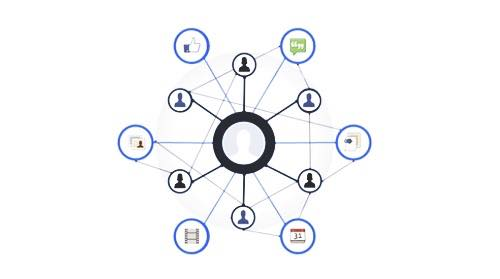
\includegraphics[scale=0.6]{social_graph.jpg}
\caption{Illustration du graphe social d'un utilisateur lambda.}
\end{center}
\end{figure}

\subsection{Accès aux données et restrictions}
Avant de pouvoir récupérer les données du service, il faut d'abord s'identifier auprès du serveur.Cela s'utilise à l'aide d'une technologie connue pour la gestion de l'authentification :\textbf{OAuth 2.0.}\footnote{http://oauth.net/}. \\
Pour ce faire, il faut au préalable être inscrit auprès de Facebook developpers\footnote{\url{http://developers.facebook.com}} et de l'application qu'on souhaite développer et ce en se rendant à la page correspondante.
Après cela il faut générer le jeton d'accès.
Cela se fait à l'aide des clés de l'application fournies par Facebook.

\begin{figure}[!h]
\begin{center}

\includegraphics[scale=0.4]{web2c_app.png}
\caption{Récupération des clés de notre application.}
\label{ID_web2c}
\end{center}
\end{figure}

 Une fois qu'on tape l'url suivant : 
 \url{https://graph.facebook.com/oauth/access_token?client_id=APP_ID&client_secret=APP_SECRET&grant_type=cli}\\
 en remplaçant respectivement $APP\_ID$ et $APP\_SECRET$ par l'id de l'application et la clef secrète de l'application, on récupère le jeton d'accès qui permettra à l'application de s'identifier auprès du serveur.\\
 
\begin{figure}[!h]
\begin{center}
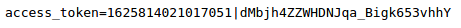
\includegraphics[scale=0.6]{token_access.png}
\caption{Récupération du jeton d'accès.}
\end{center}
\end{figure}

\subsection{Récupération et forme des données}
Une fois le jeton d'accès récupéré, nous pouvons parcourir notre graphe et exécuter des requêtes sur ce dernier. Une fois les requêtes correctement reçues par le serveur, celui-ci renvera les données de réponse au format $JSON$. \\
Par exemple, la requête d'accès aux informations publiques de Mark Zuckerberg, le co-fondateur de facebook via l'url suivant \url{http://graph.facebook.com/68310606562} où est l'id de ce dernier, nous retournera ce qui suit : 

\begin{verbatim}
{
   "id": "68310606562",
   "name": "Mark Zuckerberg",
   "picture": "http://profile.ak.fbcdn.net/hprofile-ak-snc4/502
   70_68310606562_2720435_s.jpg",
   "link": "http://www.facebook.com/markzuckerberg",
   "category": "Public figure",
   "likes": 3711466,
   "website": "www.facebook.com",
   "username": "markzuckerberg",
   "personal_interests": "openness,

}
\end{verbatim}
Nous pouvons rajouter à la fin de l'url qui précède \textbf{$/videos$} pour accéder aux vidéos du co-fondateur de Facebook. Nous pouvons faire pareil pour plusieurs objets : $friends$, $photos$, $likes$..
Il est à retenir que l'identifiant permet de définir de façon unique un objet dans l'API Facebook. C'est une valeur numérique incrémentée à chaque création d'un nouvel objet qu'il s'agisse d'un profil, d'une page, d'une application, etc. \\

\subsection{Données récupérables}
Facebook contient une panoplie d'informations récupérables sous forme de données JSON à condition d'avoir le droit d'accès à ses informations. Voici une liste non-exhaustive des données récuperables via l'Open Graph API : \\
\begin{itemize}
\item \textbf{Données de l’utilisateur :} nom, id, date de création, le nombre d'amis, la liste d'amis, etc.
\item  \textbf{Publications :} statuts, check-in, photos, vidéos, etc.
\item  \textbf{Les actions des utilisateurs :} les pages aimées, publications commentées, etc.
Données des lieux les lieux enregistrés par facebok recensent aussi plusieurs informations à savoir le nom,
les coordonnées, le pays, la ville, etc.
\end{itemize}


\section{Twitter}
    \subsection{Rappels généraux}
        Avant de présenter l'API de Twitter, il nous semble nécessaire de revenir sur le fonctionnement général du service. 
        
        Créé en 2006, Twitter\footnote{\url{https://twitter.com/}} est un service d'échange de messages courts\footnote{144 caractères pour être précis}, appelés \emph{tweets}, entre ses utilisateurs.
        Chaque utilisateur peut en suivre (\emph{follow}) d'autres, afin de rester informé de leur actualité.
        Il est également possible de \emph{retweeter} un message - c'est à dire le rediffuser sur son flux d'actualité personnel afin de le communiquer à ses \emph{followers}.
        On peut également répondre à un \emph{tweet}, ce qui créera un fil de discussion auquel différents participants peuvent se joindre.
        Outre du texte, un \emph{tweet} peut contenir une URL (pointant vers une image, une vidéo, un article ou autre) - dont le contenu sera prévisualisable sur le site et les diverses autres applications officielles - mais aussi des \emph{hashtags}, à savoir des mots-clé précédés par le symbole \#, et des \emph{mentions}, soit le nom d'un autre utilisateur précédé par le symbole @.
        
        L'intérêt des \emph{hashtags} et \emph{mentions} est d'être interactifs. Depuis les applications officielles, il est ainsi possible de suivre tous les \emph{tweets} lié à un \emph{hashtag} particulier, d'accéder directement au profil d'une personne \emph{mentionnée} ou encore de recevoir des notifications lorsque c'est notre cas.
    
    \subsection{Description des API}
        Twitter fournit deux API pour communiquer avec le service :
        \begin{description}
            
            \item[L'API REST:] Semblable à ce que l'on trouve sur Facebook, cette API permet de récupérer des données selon des critères définis, de façon "figée". 
            C'est à dire que le client envoie une requête serveur, qui renverra une réponse, et c'est tout.
            La quantité de requêtes est limitée à 450 pour 15 minutes.
            
            \item[L'API Streaming:] À l'inverse le l'API REST, l'API Streaming fournit un flux continu de données, ce qui est très pratique pour récupérer un fil de \emph{tweets} en direct.
            Cette API elle même permet d'accéder à trois flux de données :
            
            \begin{description}
                \item[Public Stream], qui fournit un accès à des données accessibles à tous ;
                \item[User Stream], qui fournit un accès à des données accessibles par l'utilisateur courant;
                \item[Site Stream], une version multi-utilisateur et \textbf{encore en bêta} de \emph{User Stream}.
            \end{description}
            
            La quantité de messages récupérés ne doit cependant pas excéder 1\% de tous ceux échangés à un instant T.
            
        \end{description}
        
        Il est possible de tester le fonctionnement des différentes API à l'adresse suivante : \url{https://dev.twitter.com/rest/tools/console}
        
    \subsection{Accès aux données \& restrictions}
        Avant de pouvoir récupérer les données du service, il faut s'identifier auprès du serveur à l'aide du protocole \textbf{OAuth}\footnote{http://oauth.net/}.
        Pour ce faire, il faut au préalable nécessaire d'enregistrer auprès de Twitter l'application que l'on souhaite développer, en se rendant à la page correspondante\footnote{\url{http://apps.twitter.com/new}} avec un compte Twitter existant.
        Ensuite, il faut encore générer les jetons d'accès et clés API à récupérer afin que l'application puisse s'authentifier auprès du serveur.
        
        Une fois que les requêtes correctement reçues par le serveur, celui-ci renverra les données de réponse au format \emph{JSON}.
        
    \subsection{Récupération des données}
        De nombreuses bibliothèques existent pour se connecter au service et en récupérer des données facilement.
        La documentation de l'API en recense d'ailleurs pour un grand nombre de langages\footnote{\url{https://dev.twitter.com/overview/api/twitter-libraries}}.
        
        \lstset{style=RubyStyle}
        \begin{lstlisting}[caption=Exemple de recherche sur l'API Streaming avec la \emph{RubyGem} \textbf{TweetStream} (\url{https://github.com/tweetstream/tweetstream})]
require 'tweetstream'

TweetStream.configure do |config|
	config.consumer_key       = 'MY_KEY'
	config.consumer_secret    = 'MY_SECRET'
	config.oauth_token        = 'MY_TOKEN'
	config.oauth_token_secret = 'MY_SECRET_TOKEN'
	config.auth_method        = :oauth
end

#Recherche via keywords
TweetStream::Client.new.track('keyword 1', 'keyword 2') do |status|
	puts "#{status.text}"
end
        \end{lstlisting}
        
        
    \subsection{Données récupérables}
        L'intégralité des données récupérables via les différentes API peut être trouvée dans sa documentation officielle\footnote{\url{https://dev.twitter.com/overview/api}}.
        En voici un recensement non-exhaustif.
        
        \subsubsection{Données de l'utilisateur}
            On peut récupérer pêle-mêle : le nom, l'identifiant, la date de création, le nombre de followers, les relation avec l'utilisateur courant (est-ce un \emph{follower} ? Le suit-il ?), l'activation ou non de la géolocalisation, l'adhésion à certaines communautés (de traduction notamment), la localisation, l'apparence du profil (avatar, bannière, etc), les derniers \emph{tweets}, etc.
            
        \subsubsection{Données des \emph{tweets}}
            De même, un grand nombre d'informations liées aux \emph{tweets} sont accessible : le contenu du message, les coordonnées (la géolocalisation de l'auteur au moment de l'envoi, si l'option est activée), la date d'envoi, l'identifiant du message, l'état de la discussion, la langue du message, un lien éventuel avec un lieu précis (référencé par Twitter), la présence de contenu sensible, les informations de l'auteur, l'existence de plaintes DMCA\footnote{(Du nom du \emph{Digital Millennium Copyright Act}) Plaintes liées aux infractions à la propriété intellectuelle aux États-Unis. Voir la page Wikipédia : \url{https://fr.wikipedia.org/wiki/Digital_Millennium_Copyright_Act}} à l'encontre du message, si le message est filtré dans certains pays, etc.
            
        \subsubsection{Données des lieux}
            Les lieux enregistrés par Twitter recensent aussi plusieurs informations  : son nom, ses coordonnées (les extrémités d'une boîte l'encadrant), son pays, sont type (ville, musée), une url, son adresse physique, sa ville, un numéro de téléphone de contact, etc.
        
        \subsubsection{Données des entités supplémentaires}
            On peut aussi récupérés des informations liées aux différentes entités éventuellement présentes dans le \emph{tweet}, tels les \emph{hashtags}, médias (images, vidéos, ...), URL et mentions d'autres utilisateurs.
        
        
        
        
        
        
        